%&pdflatex
\documentclass[review]{elsarticle}
\journal{European Journal of Mechanics - B/Fluids}

\usepackage{graphicx}
\usepackage{amssymb, amsmath}
\usepackage{fullpage}
\usepackage{hyperref}
\usepackage{natbib}

%%% lemmas
\usepackage{amsthm}
\newtheorem{lemma}{Lemma}

%%% line numbers
\usepackage{lineno}

%%% breaking long formulas
\allowdisplaybreaks[3]

%%% URL in bibliography
\usepackage{url}

%%% right alignment of pics in the appendix
\usepackage[export]{adjustbox}

%\renewcommand{\includegraphics}{\relax}

%%% subfigures
\usepackage[skip=0pt]{subcaption}
\captionsetup{compatibility=false, subrefformat=parens}

%%% advanced subfigures
\usepackage{floatrow}
\DeclareFloatSeparators{mywidth}{\hspace{-15pt}}
\floatsetup[subfigure]{
    style=plain,
    capbesideposition={left,top},
    capbesidewidth=.5cm,
    capbesidesep=mywidth
}

%%% abbreviations for the manuscript
\newcommand{\Kn}{\mbox{\textit{Kn}}}
\newcommand{\NS}{N\!S}
\newcommand{\dd}{\mathrm{d}}
\newcommand{\der}[2][]{\frac{\dd#1}{\dd#2}}
\newcommand{\pder}[2][]{\frac{\partial#1}{\partial#2}}
\newcommand{\pderdual}[2][]{\frac{\partial^2#1}{\partial#2^2}}
\newcommand{\pderder}[3][]{\frac{\partial^2#1}{\partial#2\partial#3}}
\newcommand{\Pder}[2][]{\partial#1/\partial#2}
\newcommand{\dzeta}{\boldsymbol{\dd\zeta}}
\newcommand{\bzeta}{\boldsymbol{\zeta}}
\newcommand{\bh}{\boldsymbol{h}}
\newcommand{\Nu}{\mathcal{N}}
\newcommand{\Mu}{\mathcal{M}}
\newcommand{\OO}[1]{O\left(#1\right)}
\newcommand{\Set}[2]{\{\,{#1}:{#2}\,\}}

%%% abbreviations for the appendix
\newcommand{\B}{\ensuremath{\mathcal{B}^{(4)}}}
\newcommand{\Q}{\ensuremath{\mathcal{Q}^{(0)}}}
\newcommand{\T}[1]{\ensuremath{\mathcal{T}^{(#1)}}}
\newcommand{\TT}{\ensuremath{\tilde{\mathcal{T}}^{(0)}}}
\newcommand{\QQ}{\ensuremath{\tilde{\mathcal{Q}}^{(0)}}}
\newcommand{\ZD}[2]{\zeta_{#1}\delta_{#2}}
\newcommand{\ZZD}[3]{\zeta_{#1}\zeta_{#2}\delta_{#3}}
\newcommand{\ZZZ}{\zeta_i\zeta_j\zeta_k}
\newcommand{\ZZZZ}{\zeta_i\zeta_j\zeta_k\zeta_l}
\newcommand{\DD}[2]{\delta_{#1}\delta_{#2}}

\begin{document}

\begin{frontmatter}

\title{
    Numerical analysis of the nonlinear plane Couette-flow problem of a rarefied gas for hard-sphere molecules
}

\author{Oleg Rogozin}
\ead{oleg.rogozin@phystech.edu}
\address{
    Moscow Institute of Physics and Technology,
    9 Institutskiy pereulok, Dolgoprudny,
    Moskovskaya obl., Russian Federation
}

\begin{keyword}
   Couette flow \sep
   rarefied gas dynamics \sep
   Boltzmann equation \sep
   asymptotic analysis \sep
   projection method \sep
   OpenFOAM \sep
   DSMC
\end{keyword}

%\pacs{
%    47.45.Ab,   % Kinetic theory of gases
%    47.11.Df,   % Finite volume methods
%    47.15.-x,   % Laminar flows
%    51.10.+y    % Kinetic and transport theory of gases
%}

\begin{abstract}
    The plane Couette flow of a rarefied gas is investigated on the basis of the Boltzmann equation
    over the wide range of Knudsen and Mach numbers.
    The velocity distribution function as well as its first thirteen moments is obtained from
    the accurate numerical solution based on the projection discrete-velocity method
    extended for nonuniform rectangular velocity grids.
    The DSMC simulation is used to reinforce the obtained results.
    The nonlinear Hilbert-type asymptotic solution for a slightly rarefied gas
    is constructed and also included in the comparison.
    For this purpose, some additional transport coefficients for hard-sphere molecules are evaluated.
\end{abstract}

\end{frontmatter}

\linenumbers

\section{Introduction}

%%% Linear problem
The steady state of a gas between two parallel plates with the same temperature
and opposite velocities is one of the most fundamental boundary-value problems of kinetic theory.
The linear Couette-flow problem, described by the linearized Boltzmann equation,
has a long history of applied approximate methods~\citep{Willis1962}.
\citet{Ohwada1990} have solved it with high accuracy for hard-sphere molecules.
The latter solution is often used for validation of numerical methods~\citep[see e.g.][]{Fan2001,Aidun2010}.

%%% Nonlinear problem
The nonlinear problem is also studied extensively~\citep{Garzo2003}.
Despite the remarkable progress in the development of deterministic numerical methods
in the recent years~\citep[see e.g.][]{Dimarco2014,Mieussens2014},
which can provide more accurate solutions compared to stochastic techniques,
it is the direct simulation Monte-Carlo (DSMC), with its inherent statistical noise,
that serves as the reference solution~\citep[see e.g.][]{Cercignani1994,Struchtrup2009,Agrawal2014}.
The present study is aimed to obtain a high-accuracy deterministic solution
of the nonlinear problem for various external parameters.

%%% The primary numeric method
The projection-interpolation method of discrete velocities is chosen for
evaluation of the Boltzmann integral~\citep{Tcheremissine1998, Tcheremissine2006}.
With this technique, velocities after impact that do not hit the grid
are projected to the adjacent grid nodes in such a way that mass, momentum, and energy are conserved.
The gain term of the Boltzmann integral is interpolated in such a way that
the discrete collision operator from the Maxwell distribution is strictly equal to zero.
The projection-interpolation method of evaluation of the collision integral
provides the second order approximation along each axis for a smooth distribution function~\citep{Anikin2012}.
However, there are discontinuities and large variations for real boundary-value problems,
which significantly increase the error of computation on a uniform velocity grid.
Therefore, nonuniform velocity grids, condensing in areas of large variation
of the distribution function, should be used to obtain a high-accuracy solution.
For uniform grids, two projection nodes are enough to satisfy the conservation laws,
otherwise it is necessary to resort to the multipoint projection stencils~\citep{Dodulad2012}.
In the present paper, an extension of the projection method for nonuniform grids is employed.
The author hopes that the proposed method can yield the most accurate results
among the existing numerical methods for the considered problem.

%%% Asymptotic solution
Fluid-dynamic-type equations together with special boundary conditions
are often used to find an approximate solution for small Knudsen numbers.
For example, the Navier--Stokes equations with the slip boundary conditions~\citep{Ohwada1989a}
give an opportunity to construct the simplest solution~\citep{Sharipov2000}.
To take into account the next order of gas rarefaction in the Chapman--Enskog expansion,
the Burnett~\citep{Reese2003} and super-Burnett~\citep{Agrawal2014} equations can be considered.
The Grad's moment method and its modifications are also applied~\citep{Struchtrup2009}.
However, to obtain a rigorous asymptotic solution of the Boltzmann equation,
the Hilbert expansion along with the systematic examination of the viscous boundary and Knudsen layers
should be carried out. \citet{Sone2000} have introduced the general approach
for construction of the asymptotic solution for finite Mach numbers.
In the present study, this approach is applied to the plane Couette-flow problem.
The obtained results is also used to verify the direct numerical solution
of the Boltzmann equation for small Knudsen numbers.

\section{Formulation of the problem}

Consider a monatomic ideal gas confined between two infinite parallel plates
with complete diffuse reflection.
A plane Couette flow is formed by motion of the plates relative to each other
with the longitudinal velocity along the \(x\) axis,
while their temperatures remain equal and constant.
The \(y\) axis is normal to the plates separated by distance \(L\).

In the present paper, we deal with dimensionless quantities. The macroscopic variables
have the following form: \(p_{ij}p^{(0)}\) is the stress tensor, \(TT^{(0)}\) is the temperature,
\(\rho p^{(0)}/RT^{(0)}\) is the density, \(v_i(2RT^{(0)})^{1/2}\) is the velocity
and \(q_ip^{(0)}(2RT^{(0)})^{1/2}\) is the heat-flow vector.
The specific gas constant \(R = k_B/m\), where \(k_B\) is the Boltzmann constant
and \(m\) is the molar mass.
Let \(L\) be a reference length and the velocities of the plates (\(y=\pm1/2\))
be equal to \((\pm\Delta{v}/2)(2RT^{(0)})^{1/2}\), respectively.
\(T^{(0)}\) is the common temperature of the plates.
\(p^{(0)}\) is selected in such a way that the average density is equal to one, i.e.
\begin{equation}\label{eq:total_mass}
    \int_{-\frac12}^\frac12\rho\dd{y} = 1.
\end{equation}

\subsection{Kinetic description}

Molecules are assumed as hard spheres, the Knudsen number is
\begin{equation}\label{eq:Kn_number}
    \Kn = \frac{\ell_0}{L} = \frac{k_BT^{(0)}}{\pi\sqrt{2} d_m^2p^{(0)}L},
\end{equation}
where \(\ell_0\) is the mean free path for the reference density \(\rho^{(0)} = p^{(0)}/R T^{(0)}\),
\(d_m\) is the diameter of molecules.
To describe an ideal gas over the wide range of Knudsen numbers
one should apply the Boltzmann equation.
Its dimensionless and time-independent form is
\begin{equation}\label{eq:Boltzmann}
    \zeta_i\pder[f]{x_i} = \frac1k J(f,f),
\end{equation}
where \(k = \Kn\sqrt{\pi}/2\) is a modified Knudsen number and
\begin{equation}\label{eq:ci}
    J(f,g) = \frac12 \int (f'g'_* + f'_*g' - fg_* - f_*g) B
    \dd \Omega(\boldsymbol{\alpha}) \dzeta_*,
\end{equation}
is the Boltzmann collision integral.
The distribution function \(f(x_i,\zeta_i)(2p^{(0)})/(2RT^{(0)})^{5/2}\) is defined
in the space \([x_iL, \zeta_i(2RT^{(0)})^{1/2}]\).
\(\dd \Omega(\boldsymbol{\alpha})\) is an element of solid angle in the direction of the unit vector \(\alpha_i\),
determining the velocities after impact:
\begin{equation}\label{eq:after_impact}
    \zeta'_i = \zeta_i + \alpha_i\alpha_j(\zeta_{j*}-\zeta_j), \quad
    \zeta'_{i*} = \zeta_{i*} - \alpha_i\alpha_j(\zeta_{j*}-\zeta_j).
\end{equation}
For the hard-sphere model,
\begin{equation}\label{eq:ci_kernel}
    B = \frac{|\alpha_i(\zeta_{i*}-\zeta_i)|}{4\sqrt{2\pi}}.
\end{equation}

The Maxwell-type boundary condition with diffuse reflection is used at \(y=1/2\), i.e.
\begin{equation}\label{eq:diffuse_bc}
    f(\zeta_x,\zeta_y,\zeta_z) = \frac2{\pi} \exp\left[-\left(\zeta_x-\frac{\Delta{v}}{2}\right)^2-\zeta_y^2-\zeta_z^2\right]
        \int_{\zeta_{*y}>0}\zeta_{*y} f_* \dzeta_*, \quad \zeta_y<0.
\end{equation}
The following symmetry condition is imposed at \(y=0\):
\begin{equation}\label{eq:specular_bc}
    f(\zeta_x,\zeta_y,\zeta_z) = f(-\zeta_x,-\zeta_y,\zeta_z), \quad \zeta_y>0.
\end{equation}

The nondimensional macroscopic variables are calculated by integrating the distribution function:
\begin{equation}\label{eq:macro}
    \begin{gathered}
    \rho = \int f \dzeta, \quad
    v_i = \frac1{\rho} \int \zeta_i f \dzeta, \\
    T = \frac{2}{3\rho}\int(\zeta_i-v_i)^2 f \dzeta, \quad
    q_i = \int(\zeta_i-v_i)(\zeta_j-v_j)^2 f \dzeta, \\
    p_{ij} = 2 \int(\zeta_i-v_i)(\zeta_j-v_j) f \dzeta,
        \quad p = p_{ii}/3 = \rho T.
    \end{gathered}
\end{equation}

\subsection{Linearization of the problem}

Linearized Boltzmann equation
\begin{equation}\label{eq:linear_Boltzmann}
    \zeta_i \pder[\phi]{x_i} = \frac1k \mathcal{L}(\phi),
\end{equation}
with the linearized collision operator
\begin{equation}\label{eq:linear_ci}
    \mathcal{L}(\phi) = \int E_*(\phi'+\phi'_*-\phi-\phi_*) B
    \dd \Omega(\boldsymbol{\alpha}) \dzeta_*
\end{equation}
holds for a gas that deviates only slightly from an equilibrium state, i.e.
\begin{equation}\label{eq:linear_condition}
    \phi = \frac{f}{E} - 1 \ll 1, \quad E(\zeta) = \frac1{\pi^{3/2}}\exp\left(-\zeta^2\right).
\end{equation}
Perturbed local Maxwell distribution
\begin{equation}\label{eq:linear_maxwellian}
    \phi_e = \omega + 2\zeta_i v_i + \left(\zeta_i^2-\frac32\right)\tau
\end{equation}
is expressed in terms of the corresponding perturbed macroscopic variables:
\begin{equation}\label{eq:perturbed_variables}
    \omega = \rho-1, \quad \tau = T-1, \quad P = p-1, \quad P_{ij} = p_{ij}-\delta_{ij},
\end{equation}
where \(\delta_{ij}\) is the Kronecker delta function.

The Couette-flow problem is linearized when \(\Delta{v}\ll 1\).
The desired distribution function can be expressed in the following form:
\begin{equation}\label{eq:linear_solution}
    \phi = \Delta{v} \zeta_x \Phi(y,\zeta_y,\zeta), \quad \zeta = \sqrt{\zeta_i^2},
\end{equation}
Substituting~\eqref{eq:linear_solution} into~\eqref{eq:linear_Boltzmann}, we obtain
\begin{equation}\label{eq:linear_equation}
    \zeta_y \pder[\Phi]{y} = \frac1{k\zeta_x}\mathcal{L}(\zeta_x\Phi)
\end{equation}
with the following boundary conditions:
\begin{equation}\label{eq:linear_bc}
    \Phi_-(1/2,\zeta_y,\zeta) = 1, \quad \Phi_+(0,\zeta_y,\zeta) = -\Phi_-(0,-\zeta_y,\zeta),
\end{equation}
where \(\Phi_\pm = \Phi(\zeta_y \gtrless 0)\).
The perturbed macroscopic variables are expressed as
\begin{equation}\label{eq:linear_macro}
    \frac{P_{xy}}{\Delta{v}} = 2\int \zeta_x^2 \zeta_y \Phi E\dzeta, \quad
    \frac{v_x}{\Delta{v}} = \int \zeta_x^2 \Phi E\dzeta, \quad
    \frac{q_x}{\Delta{v}} = \int \zeta_x^2 \zeta^2 \Phi E\dzeta - \frac52 \frac{v_x}{\Delta{v}}.
\end{equation}
Other variables from~\eqref{eq:macro} remain constant in the linear case.

\section{Outline of the methods for the linear problem}

For \(k\to\infty\), we obtain the collisionless linearized Boltzmann equation \(\zeta_y\Pder[\Phi]{y} = 0\),
which has a simple solution as a combination of two different half-Maxwellians, i.e. \(\Phi_\pm = \mp 1\).
It gives
\begin{gather}\label{eq:linear_free_macro}
    \frac{P_{xy}}{\Delta{v}} = -\frac1{\sqrt{\pi}}, \quad v_x = q_x = 0.
\end{gather}

For small \(k\), there is a Grad--Hilbert solution~\citep[see e.g.][]{Ohwada1990, Sone2007}:
\begin{equation}\label{eq:small_solution}
    \Phi = \frac{2y - \zeta_y \mathcal{B}(\zeta) k}{1-2k_0k},
\end{equation}
where special function \(\mathcal{B}(\zeta)\) is defined from the integral equation
\begin{equation}\label{eq:transport_B}
    \mathcal{L}\left[\left(\zeta_i\zeta_j-\frac{\zeta^2}3\delta_{ij}\right) \mathcal{B}(\zeta)\right]
        = -2\left(\zeta_i\zeta_j-\frac{\zeta^2}3\delta_{ij}\right).
\end{equation}
The solution~\eqref{eq:small_solution} does not satisfy the boundary conditions~\eqref{eq:linear_bc},
therefore, it is corrected in the Knudsen layer. Finally, we have the following asymptotic solution:
\begin{equation}\label{eq:small_macro}
    \frac{P_{xy}}{\Delta{v}} = - \frac{\gamma_1 k}{1-2k_0k}, \quad
    \frac{v_x}{\Delta{v}} = \frac{y - (Y_0^--Y_0^+)k}{1-2k_0k}, \quad
    \frac{q_x}{\Delta{v}} = \frac{(H_A^--H_A^+)k}{1-2k_0k},
\end{equation}
where, for hard-sphere molecules,
\begin{equation}\label{eq:gamma_1}
    \gamma_1 = \frac{8}{15\sqrt{\pi}}\int_0^\infty \zeta^6 \mathcal{B}(\zeta)E\dd\zeta = 1.270042427
\end{equation}
is the viscosity coefficient and \(k_0 = -1.25395\)~\citep{Takata2015} is the slip coefficient.
The Knudsen-layer functions \(K^\pm = Y_0^\pm, H_A^\pm\) are defined as follows:
\begin{equation}\label{eq:linear_knudsen_functions}
     K^\pm = K(\eta_\pm), \quad \eta_\pm = \frac{1 \mp 2y}{2k}.
\end{equation}
For hard-sphere molecules, \(Y_0(\eta)\), \(H_A(\eta)\)
are tabulated in~\citet{Ohwada1989a, Sone2002, Sone2007, Takata2015}.
This asymptotic solution assumes that the Knudsen layers of the both plates are not intersected.
In other words, the terms as \(\exp(-1/k)\) are neglected.

In case of arbitrary \(k\), the solution can be obtained by numerical analysis.
\citet{Ohwada1990} have carefully accomplished it for the hard-sphere model.

For comparison, consider also a solution of the widely used BKW (Boltzmann--Krook--Welander) equation,
whose linearized form of collision integral
\begin{equation}\label{eq:linear_bkw}
    \mathcal{L}(\phi) = -\phi + \omega + 2\zeta_i v_i + \left(\zeta_i^2-\frac32\right)\tau
\end{equation}
leads to the differential equation
\begin{equation}\label{eq:linear_bkw_equation}
    \zeta_y \pder[\Phi]{y} = \frac1{k}\left( \frac{2v_x}{\Delta{v}} - \Phi \right).
\end{equation}
Its solution can be written in the following form~\citep{Willis1962}:
\begin{equation}\label{eq:bkw_solution}
    \Phi_\pm = \mp \exp\left(\mp\frac{\eta_\mp}{\zeta_y}\right) +
        \int_{\mp\frac12}^y \frac1{k\zeta_y} \exp \left(-\frac{y-s}{k\zeta_y}\right) g(s) \dd{s},
\end{equation}
where \(g(y) = 2v_x/\Delta v\) is found from the Fredholm integral equation of the second kind
\begin{equation}\label{eq:bkw_g_equation}
    \sqrt{\pi} g(y) = \mathcal{T}_0^+ - \mathcal{T}_0^-
        + \frac1k \int_0^{\frac12} \left[ \mathcal{T}_{-1}\left(\frac{|y-s|}{k}\right)
        - \mathcal{T}_{-1}\left(\frac{y+s}{k}\right) \right] g(s) \dd{s}.
\end{equation}
Here, \(\mathcal{T}_n(s)\) are special Abramowitz functions~\citep{Abramowitz1972}:
\begin{equation}\label{eq:Abramowitz}
    \mathcal{T}_n(s) = \int_0^\infty t^n \exp\left(-t^2-\frac{s}{t}\right) \dd t,
    \quad s\ge0, \quad n \in \mathbb{Z}.
\end{equation}
The remaining macroscopic variables are calculated as follows:
\begin{gather}
    \frac{P_{xy}}{\Delta v} = -\frac{2k}{\sqrt{\pi}} \left(
        \mathcal{T}_2(0)-\mathcal{T}_2\left(\frac1k\right)
        + \frac1k\int_0^{\frac12}\left[
            \mathcal{T}_1\left(\frac{1-2s}{2k}\right)-\mathcal{T}_1\left(\frac{1+2s}{2k}\right)
        \right]g(s)\dd{s}
        \right), \label{eq:bkw_macro_Pxy} \\
    \begin{aligned}
    \frac{q_x}{\Delta v} = \frac1{2\sqrt{\pi}}&\left(
        \mathcal{T}_2\left(\frac{1-2s}{2k}\right) - \mathcal{T}_2\left(\frac{1+2s}{2k}\right)\right. \\
        &+\left. \frac1k\int_0^{\frac12}\left[
            \mathcal{T}_1\left(\frac{|y-s|}k\right)-\mathcal{T}_1\left(\frac{y+s}k\right)
        \right]g(s)\dd{s}
        \right) - \frac{g(y)}4.
    \end{aligned} \label{eq:bkw_macro_qx}
\end{gather}

\section{Outline of the methods for the nonlinear problem}

\subsection{Free molecular solution}

Collisionless Boltzmann equation, as well as in the linearized case,
has a solution as a combination of two different half-Maxwellians:
\begin{equation}\label{eq:free_solution}
    f^\pm = f(\zeta_y \gtrless 0) =
        \frac1{\pi\sqrt{\pi}} \exp\left[-\left(\zeta_x\pm\frac{\Delta{v}}2\right)^2 - \zeta_y^2 - \zeta_z^2\right],
\end{equation}
which supplements Eqs.~\eqref{eq:linear_free_macro} with the following values of the macroscopic variables:
\begin{equation}\label{eq:free_macro}
    \frac{\tau}{(\Delta{v})^2} = \frac16, \quad q_y = 0, \quad
    \frac{P_{xx}}{(\Delta{v})^2} = \frac12, \quad P_{yy} = P_{zz} = 0.
\end{equation}

\subsection{Navier--Stokes equations}\label{sec:Navier-Stokes}

For the Couette-flow problem, the conservation equations degenerate into
\begin{equation}\label{eq:conservation_laws}
    \pder[p]{y} = 0, \quad \pder[p_{xy}]{y} = 0, \quad \pder{y}(v_x p_{xy} + q_y) = 0.
\end{equation}
Substituting Newton's and Fourier's laws,
\begin{equation}\label{eq:Newton-Fourier}
    p_{xy} = -\gamma_1 k\sqrt{T}\pder[v_x]{y}, \quad q_y = -\frac54\gamma_2 k\sqrt{T}\pder[T]{y},
\end{equation}
into Eqs.~\eqref{eq:conservation_laws}, we obtain a system of differential equations
\begin{equation}\label{eq:Navier-Stokes}
    \pder{y}\left(\sqrt{T}\pder[v_x]{y}\right) = 0, \quad
    \sqrt{T}\left(\pder[v_x]{y}\right)^2 + \frac54\frac{\gamma_2}{\gamma_1}\pder{y}\left(\sqrt{T}\pder[T]{y}\right) = 0,
\end{equation}
which are usually solved with the nonslip boundary conditions at \(y=1/2\):
\begin{equation}\label{eq:nonslip_bc}
    v_x = \frac{\Delta{v}}2, \quad T = 1.
\end{equation}
Incidentally, \(\gamma_2 = 1.922284066\) is the thermal conductivity coefficient of a hard-sphere gas.
The constant pressure \(p\) is calculated from the total mass of the gas (see~\eqref{eq:total_mass}):
\begin{equation}\label{eq:constant_pressure}
    p = \left( 2\int_{0}^\frac12\frac{\dd{y}}{T} \right)^{-1}.
\end{equation}

\subsection{Asymptotic analysis for small Knudsen numbers}

The Navier--Stokes equations can be obtained from the Chapman--Enskog expansion
and, in essence, describe some kind of disturbance of the equilibrium Maxwellian state.
To obtain a rigorous asymptotic solution for small \(k\),
one should refer to the Hilbert expansion in connection with the
viscous boundary and Knudsen layers~\citep{Sone2000, Sone2002}.

Expanding macroscopic variables \(h = \rho, v_i, T, \dots\) into a power series of \(k\), i.e.
\begin{equation}\label{eq:hilbert_expansion}
    h = h_0 + h_1k + h_2k^2 + \cdots,
\end{equation}
we obtain, in the context of the plane Couette-flow problem, the following set of equations up to the first order:
\begin{gather}
    \pder{y}\left( \sqrt{T_0}\pder[v_{x0}]{y} \right) = 0, \label{eq:Hilbert_U0}\\
    \sqrt{T_0}\left( \pder[v_{x0}]{y}\right)^2 + \frac{5\gamma_2}{4\gamma_1}\pder{y}\left(\sqrt{T_0}\pder[T_0]{y} \right) = 0, \label{eq:Hilbert_T0}\\
    \pder{y}\left( \sqrt{T_0}\pder[v_{x1}]{y} + \frac{T_1}{2\sqrt{T_0}}\pder[v_{x0}]{y} \right) = 0, \label{eq:Hilbert_U1}\\
    \left( 2\sqrt{T_0}\pder[v_{x1}]{y} + \frac{T_1}{2\sqrt{T_0}}\pder[v_{x0}]{y} \right) \pder[v_{x0}]{y}
        + \frac{5\gamma_2}{4\gamma_1} \pder{y}\left( \sqrt{T_0}\pder[T_1]{y} + \frac{T_1}{2\sqrt{T_0}}\pder[T_0]{y} \right) = 0. \label{eq:Hilbert_T1}
\end{gather}
The leading-order equations~\eqref{eq:Hilbert_U0}--\eqref{eq:Hilbert_T0}
is seen to coincide with the Navier--Stokes equations~\eqref{eq:Navier-Stokes}.
The pressure is constant up to the first order:
\begin{gather}
    \pder[p_0]{y} = 0, \quad \pder[p_1]{y} = 0, \label{eq:hilbert_p0_p1} \\
    \frac{3p_0}{2}\pder[p_2]{y}
        + \pder{y}\left[ \gamma_3 T_0 \pderdual[T_0]{y} + \gamma_7\left(\pder[T_0]{y}\right)^2 \right]
        + \pder{y}\left[ (\gamma_8-2\gamma_9)T_0\left(\pder[v_{x0}]{y}\right)^2 \right] = 0, \label{eq:hilbert_p2}
\end{gather}
where
\begin{equation}\label{eq:hilbert_expansion_p}
    p_0 = \rho_0 T_0, \quad
    p_1 = \rho_1 T_0 + \rho_0 T_1, \quad
    p_2 = \rho_2 T_1 + \rho_1 T_1 + \rho_0 T_2.
\end{equation}

Boundary conditions at \(y=1/2\),
\begin{gather}
    v_{x0} = v_{Bx0}, \quad v_{x1} = v_{Bx1} + k_0 \frac{T_0}{p_0} \pder[v_{x0}]{y}, \label{eq:hilbert_bc_U}\\
    T_0 = T_{B0}, \quad T_1 = T_{B1} - d_1 \frac{T_0}{p_0} \pder[T_0]{y}, \label{eq:hilbert_bc_T}
\end{gather}
where \(d_1 = 2.40014\) is another slip coefficient~\citep{Takata2015},
have some freedom of the expansion in \(k\):
\begin{equation}\label{eq:hilbert_boundary_expansion}
    \frac{\Delta{v}}2 = v_{Bx} = v_{Bx0} + v_{Bx1}k, \quad 1 = T_B = T_{B0} + T_{B1}k.
\end{equation}
Putting \(T_1 = 0\) and \(v_{x1} = 0\) at \(y=1/2\), we obtain a trivial solution
for~\eqref{eq:Hilbert_U1}--\eqref{eq:Hilbert_T1}:
\begin{equation}\label{eq:hilbert_solution1}
    T_1 = 0, \quad v_{x1} = 0.
\end{equation}
Thus, we come to the Navier--Stokes equations with the following slip boundary conditions at \(y=1/2\):
\begin{equation}\label{eq:hilbert_slip_bc}
    v_{x0} = v_{Bx} + k_0 \frac{T_0}{p_0} \pder[v_{x0}]{y} k, \quad
    T_0 = T_B - d_1 \frac{T_0}{p_0} \pder[T_0]{y} k.
\end{equation}
Note that the slip boundary conditions for the linear problem, which is, for instance,
used in~\citet{Sharipov2000}, are not correct in case of finite Mach numbers.

Substituting the density \(\rho = \rho_0 + (\rho_1+\rho_{K1})k + \OO{k^2}\),
where the subscript \(K\) denotes the Knudsen-layer part of solution,
and Eqs.~\eqref{eq:hilbert_expansion_p} into Eq.~\eqref{eq:total_mass}, we obtain
\begin{equation}\label{eq:hilbert_total_mass}
    \frac12 = (p_0 + p_1k)\int_{0}^\frac12\frac{\dd y}{T_0} + \OO{k^2}.
\end{equation}
Due to~\eqref{eq:hilbert_solution1} and \(\int_{0}^{1/2}\rho_{K1}\dd{y} = \OO{k}\),
\(T_1\) and \(\rho_{K1}\) are not included in~\eqref{eq:hilbert_total_mass}.
Having the same degree of freedom in the choice of \(p_0\) and \(p_1\), put also \(p_1 = 0\).
Finally, taking into account the Knudsen-layer correction, the asymptotic solution is expressed as
\begin{gather}
    p = \left( 2\int_{0}^\frac12\frac{\dd{y}}{T_0} \right)^{-1}
        - (\Omega_1^-+\Omega_1^+ + \Theta_1^-+\Theta_1^+)\left.\pder[T_0]{y}\right|_{y=\frac12}k + \OO{k^2}, \label{eq:Hilbert_p}\\
    v_x = v_{x0} - \frac{Y_0^--Y_0^+}{p_0}T_{B0}\left.\pder[v_{x0}]{y}\right|_{y=\frac12}k + \OO{k^2}, \label{eq:Hilbert_U}\\
    T = T_0 - \frac{\Theta_1^-+\Theta_1^+}{p_0}T_{B0}\left.\pder[T_0]{y}\right|_{y=\frac12}k + \OO{k^2}, \label{eq:Hilbert_T}\\
    p_{xy} = -\gamma_1\sqrt{T_0}\pder[v_{x0}]{y}k + \OO{k^3}, \label{eq:Hilbert_Pxy}\\
    \begin{aligned}
        q_x = (H_A^--H_A^+)T_{B0}\left.\pder[v_{x0}]{y}\right|_{y=\frac12}k &+ q_{xK2}k^2 \\
        &+ \frac{T_0}{p_0}\left(\frac{\gamma_3}2 T_0 \pderdual[v_{x0}]{y}
        + 4\gamma_{10} \pder[T_0]{y}\pder[v_{x0}]{y}\right)k^2 + \OO{k^3},
    \end{aligned}\label{eq:Hilbert_Qx}\\
    q_y = -\frac54\gamma_2\sqrt{T_0}\pder[T_0]{y}k + q_{yK2}k^2 + \OO{k^3}, \label{eq:Hilbert_Qy}\\
    \begin{aligned}
    p_{xx} - p &= -\frac12 (\Omega_1^-+\Omega_1^+ + \Theta_1^-+\Theta_1^+)\left.\pder[T_0]{y}\right|_{y=\frac12}k
        + (p_{xxK2}-p_{K2})k^2 \\
        &+ \frac1{3p_0}\left[-\left(\gamma_3 T_0 \pderdual[T_0]{y} + \gamma_7\left(\pder[T_0]{y}\right)^2\right)
        + 2(\gamma_8+\gamma_9)T_0\left(\pder[v_{x0}]{y}\right)^2\right]k^2 + \OO{k^3},
    \end{aligned}\label{eq:Hilbert_Pxx}\\
    \begin{aligned}
    p_{yy} - p &= (\Omega_1^-+\Omega_1^+ + \Theta_1^-+\Theta_1^+)\left.\pder[T_0]{y}\right|_{y=\frac12}k
        + (p_{yyK2}-p_{K2})k^2 \\
        &+ \frac1{3p_0}\left[2\left(\gamma_3 T_0 \pderdual[T_0]{y} + \gamma_7\left(\pder[T_0]{y}\right)^2\right)
        + 2(\gamma_8-2\gamma_9)T_0\left(\pder[v_{x0}]{y}\right)^2\right]k^2 + \OO{k^3},
    \end{aligned}\label{eq:Hilbert_Pyy}\\
    \begin{aligned}
    p_{zz} - p &= -\frac12 (\Omega_1^-+\Omega_1^+ + \Theta_1^-+\Theta_1^+)\left.\pder[T_0]{y}\right|_{y=\frac12}k
        + (p_{zzK2}-p_{K2})k^2 \\
        &+ \frac1{3p_0}\left[-\left(\gamma_3 T_0 \pderdual[T_0]{y} + \gamma_7\left(\pder[T_0]{y}\right)^2\right)
        + 2(\gamma_9-2\gamma_8)T_0\left(\pder[v_{x0}]{y}\right)^2\right]k^2 + \OO{k^3}.
    \end{aligned}\label{eq:Hilbert_Pzz}
\end{gather}
In the above formulas, the following thermal-stress transport coefficients are used:
\begin{equation}\label{eq:gamma_tabular}
    \gamma_3 = 1.947906335, \quad \gamma_7 = 0.189201.
\end{equation}
Evaluation of the transport coefficients \(\gamma_8\), \(\gamma_9\), \(\gamma_{10}\)
for the hard-sphere model are not presented in the literature,
therefore they have been obtained by direct solution of the corresponding integral equations
(see Appendix~\ref{sec:gamma_coeffs}):
\begin{equation}\label{eq:gamma_numerical}
    \gamma_8 = 1.496(3), \quad \gamma_9 = 1.635(7), \quad \gamma_{10} = 2.463(3).
\end{equation}
The Knudsen-layer functions \(K^\pm = Y_0^\pm, \Theta_1^\pm, H_A^\pm, \Omega_1^\pm\)
are defined as follows:
\begin{equation}\label{eq:nonlinear_knudsen_functions}
     K^\pm = K\left(\frac{p_0}{T_0}\eta_\pm\right), \quad \eta_\pm = \frac{1 \mp 2y}{2k}.
\end{equation}
For hard-sphere molecules, \(\Theta_1(\eta)\) and \(\Omega_1(\eta)\)
are tabulated in~\citet{Ohwada1992, Sone2002, Sone2007, Takata2015}.
The Knudsen-layer correction of the second order is not studied in the present paper.

The presented set of equations~\eqref{eq:Hilbert_U0}--\eqref{eq:Hilbert_T0}
with the boundary conditions~\eqref{eq:hilbert_slip_bc}
is solved accurately by the finite-volume method
implemented in OpenFOAM\textregistered{}.

\subsection{Statistical simulation}

The DSMC method is the conventional numerical method in rarefied gas dynamics.
Its description is omitted in the present paper,
because it can be easily found in the literature~\citep[see e.g.][]{Bird1994, Sone2007}.
An open-source parallel solver, \verb+dsmcFoam+~\citep{Reese2010},
based on the widespread CFD toolbox OpenFOAM\textregistered{}, is used.

Numerical simulation of the hard-sphere gas between two parallel plates is carried out
in the two-dimensional space \((x,y)\) under periodic boundary conditions along the \(y\) axis.
The size of the statistical ensemble is \(2\times10^6\) for \(\Delta{v}=0.1\)
and \(2\times10^5\) for \(\Delta{v}\ge1\).
The space interval \(0<y<1/2\) is divided into uniform sections:
from 40 for \(\Kn=10\) to 100 for \(\Kn=0.1\).
The time step is chosen empirically to provide a satisfactory approximation of the macroscopic variables:
\begin{equation}\label{eq:dsmc_timestep}
    \Delta{t} = \frac{\pi}2 \frac{\sqrt{\Kn}}{1000}.
\end{equation}
In order to reduce the statistical noise, values of all macroscopic variables
are averaged over time after reaching a steady state.

\subsection{Discrete-velocity solution}

The Boltzmann equation is solved directly by symmetric splitting
into the advection equation
\begin{equation}\label{eq:split_advection}
    \pder[f]{t} + \zeta_i\pder[f]{x_i} = 0,
\end{equation}
for which a finite-volume method with an explicit second-order TVD (total variation diminishing) scheme is used,
and the space-homogeneous Boltzmann equation
\begin{equation}\label{eq:split_collisions}
    \pder[f]{t} = \frac1k J(f,f),
\end{equation}
for which the second-order projection-interpolation method of discrete velocities is used.
The main algorithm is presented in the literature~\citep[see e.g.][]{Tcheremissine1998, Tcheremissine2006, Dodulad2015}.
In the present paper, we outline the conservative method for evaluation of the Boltzmann collision integral
on nonuniform velocity grids based on the multipoint technique~\citep{Dodulad2012}.

%%% Numerical approximation
Let a regular velocity grid \(\mathcal{V} = \Set{\zeta_\gamma}{\gamma\in\Gamma}\) be constructed so that
the cubature in \(\bzeta\) space is expressed in the weighted sum
\begin{equation}\label{eq:zeta_cubature}
    \int F(\bzeta) \dzeta \approx \sum_{\gamma\in\Gamma} F_\gamma w_\gamma =
        \sum_{\gamma\in\Gamma} \hat{F_\gamma},
        \quad \sum_{\gamma\in\Gamma} w_\gamma = V_\Gamma,
        \quad F_\gamma = F(\bzeta_\gamma),
\end{equation}
where \(F\) is an arbitrary function of \(\bzeta\) (\(\hat{F_\gamma}\) is used for convenient),
\(V_\Gamma\) is the total volume of the velocity grid.
Then, the collision integral written in the symmetrized form
\begin{equation}\label{eq:symm_ci}
    \begin{aligned}
    J(f_\gamma, f_\gamma) = \frac14\int &\left[
        \delta(\bzeta-\bzeta_\gamma) + \delta(\bzeta_*-\bzeta_\gamma)
        - \delta(\bzeta'-\bzeta_\gamma) - \delta(\bzeta'_*-\bzeta_\gamma)\right] \\
        &\times(f'f'_* - ff_*)B \dd\Omega(\boldsymbol{\alpha}) \dzeta\dzeta_*,
    \end{aligned}
\end{equation}
where \(\delta(\bzeta)\) is the Dirac delta function in \(\mathbb{R}^3\),
has the following discrete analogue:
\begin{equation}\label{eq:discrete_symm_ci}
    \hat{J_\gamma} = \frac{\pi V_\Gamma^2}{\sum_{\nu\in\Nu} w_{\alpha_\nu}w_{\beta_\nu}}
        \sum_{\nu\in\Nu} \left(
            \delta_{\alpha_\nu\gamma} + \delta_{\beta_\nu\gamma}
            - \delta_{\alpha'_\nu\gamma} - \delta_{\beta'_\nu\gamma}
        \right)\left(
            \frac{w_{\alpha_\nu}w_{\beta_\nu}}{w_{\alpha'_\nu}w_{\beta'_\nu}}
            \hat{f}_{\alpha'_\nu}\hat{f}_{\beta'_\nu} - \hat{f}_{\alpha_\nu}\hat{f}_{\beta_\nu}
        \right)B_\nu.
\end{equation}
Here, \(\alpha_\nu\in\Gamma\) and \(\beta_\nu\in\Gamma\), along with \(\boldsymbol{\alpha}_\nu\),
are taken from the Korobov's lattice rule~\citep{Korobov1959, Sloan1994}
for the eight-dimensional cubature.
To ensure equal contribution of all valid values of
\(\bzeta_{\alpha_\nu}\), \(\bzeta_{\beta_\nu}\), and \(\alpha_\nu\),
the integration lattice is randomly shifted every time step.
To satisfy~\eqref{eq:total_mass} exactly, the following approximation of the Maxwell distribution is used:
\begin{equation}\label{eq:discrete_Maxwell}
    \hat{f}_{M\gamma} = \rho\left[\sum_{\alpha\in\Gamma}w_\alpha\exp
            \left(-\frac{(\bzeta_\alpha - \boldsymbol{v})^2}{T}\right)
        \right]^{-1}
        w_\gamma\exp\left(-\frac{(\bzeta_\gamma - \boldsymbol{v})^2}{T}\right).
\end{equation}

%%% Projection and interpolation
In the general case, the velocities after impact,
\(\bzeta_{\alpha'_\nu}\) and \(\bzeta_{\beta'_\nu}\), are not in \(\mathcal{V}\).
If they are replaced with the nearest grid velocities,
\(\bzeta_{\lambda_\nu}\in\mathcal{V}\) and \(\bzeta_{\mu_\nu}\in\mathcal{V}\),
the discrete collision integral~\eqref{eq:discrete_symm_ci} will not be strictly conservative,
and the discrete Maxwell distribution will not be the equilibrium state.
To resolve this issues, the following two procedures are applied in the projection-interpolation method.
First, \(\bzeta_{\alpha'_\nu}\) is projected to a set of grid nodes
\(\Set{\bzeta_{\lambda_\nu+s_a}}{a\in\Lambda}\subset\mathcal{V}\) in the following way:
\begin{equation}\label{eq:ci_projection}
    \delta_{\alpha'_\nu\gamma} = \sum_{a\in\Lambda} r_{\lambda,a}\delta_{\lambda_\nu+s_a,\gamma}.
\end{equation}
Let \(\Lambda = \Set{a}{r_{\lambda,a}\neq0}\).
The weights \(r_{\lambda,a}\) are selected to provide the conservation of mass, momentum, and energy, i.e.
\begin{equation}\label{eq:stencil_conservation}
    \sum_{a\in\Lambda} r_{\lambda,a} = 1, \quad
    \sum_{a\in\Lambda} r_{\lambda,a} \bzeta_{\lambda_\nu+s_a} = \bzeta_{\alpha'_\nu}, \quad
    \sum_{a\in\Lambda} r_{\lambda,a} \bzeta_{\lambda_\nu+s_a}^2 = \bzeta_{\alpha'_\nu}^2.
\end{equation}
Second, to satisfy
\begin{equation}\label{eq:strict_interpolation}
    J_\gamma(\hat{f}_{M\gamma}, \hat{f}_{M\gamma}) = 0,
\end{equation}
\(\hat{f}_{\alpha'_\nu}\) is interpolated in following way:
\begin{equation}\label{eq:ci_interpolation}
    \frac{\hat{f}_{\alpha'_\nu}}{w_{\alpha'_\nu}} = \prod_{a\in\Lambda}
        \left(\frac{\hat{f}_{\lambda_\nu+s_a}}{w_{\lambda_\nu+s_a}} \right)^{r_{\lambda,a}}.
\end{equation}
This type of interpolation is a high-cost approach, but it is important,
when the distribution function is close to the Maxwellian.
In practice, the exponentiation can be performed with an accuracy \(10^{-5}\),
which allows several times to speed up the calculations.
Incidentally, \eqref{eq:strict_interpolation} ensures that the H-theorem holds in the discrete form~\citep{Dodulad2013}.
For \(\bzeta_{\beta'_\nu}\) and \(\hat{f}_{\beta'_\nu}\), all formulas are similar.

%%% Description of the stencil
The set of displacement rules \(\mathcal{S} = \Set{s_a}{a\in\Lambda}\)
is called the projection stencil.
In the present paper, the most compact stencil \(|\mathcal{S}|=5\) on a rectangular velocity grid is used.
Let \(\boldsymbol{\eta} = \bzeta_{\alpha'_\nu} - \bzeta_{\lambda_\nu}\),
\(\bh_+\) and \(\bh_-\) be such minimal diagonal displacements on the grid
as \(\bh_+\) is directed in the same octant as \(\boldsymbol{\eta}\)
and \(\bh_-\) lies in the opposite one.
Then the compact 5-points scheme is constructed on the following nodes:
\begin{equation}\label{eq:stencil_nodes}
    \bzeta_{\lambda_\nu+s_0} = \bzeta_{\lambda_\nu}, \quad
    \bzeta_{\lambda_\nu+s_i} = \bzeta_{\lambda_\nu} + (\bh_+\cdot \boldsymbol{e}_i)\boldsymbol{e}_i, \quad
    \bzeta_{\lambda_\nu+s_4} = \bzeta_{\lambda_\nu} + \bh_-,
\end{equation}
where \(\boldsymbol{e}_i\) is the basis of the rectangular velocity grid.
The appropriate weights that ensure~\eqref{eq:stencil_conservation} are
\begin{equation}\label{eq:stencil_weights}
    r_{\lambda,0} = 1 - \sum_{i=1}^4 r_{\lambda,i}, \quad
    r_{\lambda,i} = \frac{(\boldsymbol{\eta} - r_{\lambda,4}\bh_-)\cdot\boldsymbol{e}_i}
        {\bh_+\cdot\boldsymbol{e}_i}, \quad
    r_{\lambda,4} = \frac{\boldsymbol{\eta}^2 - \boldsymbol{\eta}\cdot\bh_+}
        {\bh_-^2 - \bh_-\cdot\bh_+}.
\end{equation}

%%% Time-evolution scheme
Now turn to the solution of the space-homogeneous Boltzmann equation~\eqref{eq:split_collisions}.
Integrating it over the time step \(\Delta\tau\), we have
\begin{equation}\label{eq:time_scheme}
    f_\gamma(t+\Delta\tau) = f_\gamma(t) + \frac1k \int_t^{t+\Delta\tau} J_\gamma \dd\tau.
\end{equation}
Rewriting~\eqref{eq:discrete_symm_ci} as
\begin{equation}\label{eq:discrete_short_ci}
    J_\gamma = \sum_{\nu\in\Nu} \Delta_{\gamma\nu},
\end{equation}
and substituting it into~\eqref{eq:time_scheme},
we can obtain the following continuous-calculation scheme:
\begin{equation}\label{eq:continuous_scheme}
    f_\gamma^{\nu+1} = f_\gamma^\nu + \frac{\Delta\tau}{k}\Delta_{\gamma\nu}.
\end{equation}
Iteration over all \(\nu\in\Nu\) approximates~\eqref{eq:time_scheme}
with the second order.

%%% Positive property of collision integral
There is one more necessary property of the numerical algorithm:
the distribution function must always remain positive.
If there is a term in the sum~\eqref{eq:discrete_symm_ci} that violates this property,
it should be excluded from \(\Nu\).
\begin{lemma}
    If a randomly distributed set of points \(\Mu\subset\Nu\) is excluded from \(\Nu\), then
    \begin{equation*}
        \int F(\bzeta) \dzeta = \frac{\sum_{\nu\in\Nu} w_\nu}{\sum_{\nu\in\Nu,\nu\notin\Mu} w_\nu}
            \sum_{\nu\in\Nu,\nu\notin\Mu} w_\nu F_\nu + \OO{\frac{\sqrt{|\Mu|}}{|\Nu|-|\Mu|}}.
    \end{equation*}
\end{lemma}

\begin{proof}

Korobov's integration lattices provide an approximation
\begin{equation*}
    \int F(\bzeta) \dzeta = \sum_{\nu\in\Nu} w_\nu F_\nu + \OO{|\Nu|^{-p}}, \quad p\geq1.
\end{equation*}
The worst case \(p=1\) corresponds to discontinuous functions.
\begin{align*}
    \int F(\bzeta) \dzeta &= \sum_{\nu\in\Nu,\nu\notin\Mu} w_\nu F_\nu
        + \sum_{\nu\in\Mu} w_\nu F_\nu + \OO{|\Nu|^{-p}} \\
    &= \sum_{\nu\in\Nu,\nu\notin\Mu} w_\nu F_\nu
        + \frac{\sum_{\nu\in\Mu} w_\nu}{\sum_{\nu\in\Nu} w_\nu}
             \left[ \int F(\bzeta) \dzeta + \OO{\frac1{\sqrt{|\Mu|}}} \right]
        + \OO{|\Nu|^{-p}} \\
    &= \sum_{\nu\in\Nu,\nu\notin\Mu} w_\nu F_\nu
        + \frac{\sum_{\nu\in\Mu} w_\nu}{\sum_{\nu\in\Nu} w_\nu} \int F(\bzeta) \dzeta
        + \OO{\frac{\sqrt{|\Mu|}}{|\Nu|}}.
\end{align*}
We use that the convergence rate of the Monte Carlo integration is \(\OO{|\Mu|^{-1/2}}\). Hence,
\begin{equation*}
    \int F(\bzeta) \dzeta = \frac{\sum_{\nu\in\Nu} w_\nu}{\sum_{\nu\in\Nu,\nu\notin\Mu} w_\nu}
        \sum_{\nu\in\Nu,\nu\notin\Mu} w_\nu F_\nu + \OO{\frac{\sqrt{|\Mu|}}{|\Nu|-|\Mu|}}.
\end{equation*}

\end{proof}

It is easily seen that a large number of excluded collisions disturbs the integration lattice
and, therefore, the integration error can increase significantly.
To prevent this situation, one should either decrease the time step or increase \(|\Nu|\).
Another way is a modification of the interpolation technique.
The interpolation~\eqref{eq:ci_interpolation},
which strictly complies with the requirement~\eqref{eq:strict_interpolation},
can lead to a large number of excluded collisions.
Symmetric projection method, proposed in~\citet{Tcheremissine2015},
approximate~\eqref{eq:strict_interpolation} only with the second order,
but it can significantly reduce \(|\Mu|\).
In the present study, the only type of interpolation~\eqref{eq:ci_interpolation} is used.

\subsubsection{Discretization of the problem}

%%% The grid in the physical space
The physical volume of the problem (\(0<y<1/2\)) consists of \(N_x\) cells arranged in a single row.
For small \(\Kn\), the physical grid should be refined near \(y=1/2\)
due to significant variations of the solution in the thin Knudsen layer in comparison to the overall volume.

%%% The grid in the velocity
The discrete velocity space is bounded by the prolate spheroid
filled with the centred rectangular grid \(\mathcal{V}\).
The symmetry axis of the spheroid is parallel to \(x\) axis.
\(\zeta^{(\mathrm{cut})}_x\) is the semi-major axis, \(\zeta^{(\mathrm{cut})}_r\) is the semi-minor axis.
For the Couette-flow problem, the distribution function is sufficiently smooth along \(\zeta_x\) and \(\zeta_z\).
In addition, in the entire domain occupied by the gas, \(\zeta_z\) component of the distribution
differs slightly from the Maxwellian with \(v_z=0\).
For this reason, \(\zeta_z\) coordinates of \(\bzeta_\gamma\) are selected as the roots of the Hermite polynomials,
since the Gauss--Hermite quadrature is known to provide the maximum order of approximation
when integrals of the form \(\int h(s)\exp(-s^2)\dd{s}\) are evaluated.
Along \(\zeta_x\) axis, the distance between nodes is constant.
\(\zeta_y\) coordinates of \(\bzeta_\gamma\) are drift apart from \(\zeta_y=0\)
as a geometric sequence with the ratio \(r\).
This grid refinement allows significant variations of the distribution function
near \(\zeta_y=0\) to be approximated more accurately.
The weights \(w_\gamma\) are selected to provide a midpoint approximation in~\eqref{eq:zeta_cubature}.

\subsubsection{Control of accuracy}

The physical grid is refined in such a way
that the width of the marginal cell is about \(\Kn/100\).
This condition provides accuracy of the order of \(10^{-4}\) for the trapezoidal-rule quadrature
of the Knudsen-layer functions like \(Y_0(\eta)\), \(H_A(\eta)\).
For \(\Kn=100\), when the solution is similar to the constant over the physical space,
\(N_x = 30\) is sufficient for the same precision.

\begin{table}
    \centering
    \begin{tabular}{cccccccc}
        \(\Delta{v}\) & \(\zeta^{(\mathrm{cut})}_x\) & \(\zeta^{(\mathrm{cut})}_r\)
            & \(N_{\zeta_i}/2\) & \(|\mathcal{V}|\) & \(r\) & \(\Delta\zeta_x\) & \(\min(\Delta\zeta_y)\) \\[3pt]
        0.1 & 4.35 & 4.3 & (12, 26, 8)  & 15008 & 1.28 & 0.36 & 0.0020 \\
        1.0 & 4.80 & 4.5 & (14, 23, 9)  & 16872 & 1.29 & 0.34 & 0.0037 \\
        2.0 & 5.30 & 5.0 & (16, 24, 10) & 23096 & 1.28 & 0.33 & 0.0038 \\
        5.0 & 8.00 & 8.0 & (20, 26, 13) & 41520 & 1.27 & 0.40 & 0.0043 \\
    \end{tabular}
    \caption{The parameters of the velocity grid for various \(\Delta{v}\):
        \(\zeta^{(\mathrm{cut})}_x\) is the semi-major axis of the cut-off spheroid,
        \(\zeta^{(\mathrm{cut})}_r\) is the semi-minor axis,
        \(N_{\zeta_i}\) is the maximum number of nodes along each axis,
        \(|\mathcal{V}|\) is the total number of nodes,
        \(r\) is the ratio of a geometric sequence,
        \(\Delta\zeta_x\) is the distance between nodes along \(\zeta_x\) axis,
        \(\min(\Delta\zeta_y)\) is the minimum distance between nodes along \(\zeta_y\) axis.}
    \label{table:velocity_grid}
\end{table}

To assess the accuracy of the discrete approximation in the velocity space,
two opposite forms of the distribution function were considered.
First, the Grad's thirteen-moment approximation
\begin{equation}\label{eq:grad13}
    f = \frac{\rho}{(\pi T)^{3/2}}\exp\left(-\frac{c_i^2}{ T}\right)
    \left[ 1 + \frac{(p_{ij}-p\delta_{ij})c_ic_j}{pT} + \frac4{5}\frac{q_ic_i}{pT}\left(\frac{c_j^2}{T}-\frac5{2}\right) \right],
    \quad c_i = \zeta_i - v_i.
\end{equation}
is used to estimate an error for smooth functions.
Second, the combination of two different half-Maxwellians
\begin{equation}\label{eq:double_Maxwell}
    f(\zeta_y\gtrless0) = \frac{\rho^\pm}{(\pi T^\pm)^{3/2}}\exp\left(-\frac{(\zeta_x-v_x^\pm)^2+\zeta_y^2+\zeta_z^2}{T^\pm}\right).
\end{equation}
is used to simulate a discontinuity at \(\zeta_y=0\).
For small \(\Kn\) and large \(\Delta{u}\), there is a significant heating of the gas due to friction,
therefore the velocity grid should be appropriate for a velocity distribution
for both \(T=1\) near the plate and the larger temperature near the symmetry plane.
The parameters of the velocity grid sufficient to obtain accuracy of the order of \(10^{-4}\)
are presented in Table.~\ref{table:velocity_grid}.

\begin{figure}
    \centering
    \begin{subfigure}[b]{.5\linewidth}
        \includegraphics{Fig01}
        \caption{}
        \label{fig:exclusions-max}
    \end{subfigure}%
    \begin{subfigure}[b]{.5\linewidth}
        \includegraphics{Fig02}
        \caption{}
        \label{fig:exclusions-mean}
    \end{subfigure}
    \caption{The quantity \(\sqrt{|\Mu|}/|\Nu|\) versus the Knudsen number for \(\Delta{v}=5\).
        The maximum value~\subref{fig:exclusions-max} and arithmetic mean~\subref{fig:exclusions-mean}
        are taken among all physical cells and 250 successive time steps.
        The lines correspond to the various cardinality of \(\Nu\):
        from \(|\Nu| = 20011\) till \(|\Nu| = 500009\).}
    \label{fig:exclusions}
\end{figure}

The cardinality of the integration lattice \(|\Nu|\) is up to \(5\times10^5\).
While the steady state is not reached, coarser lattices are used.
From Fig.~\ref{fig:exclusions}, one can estimate an error introduced
due to the exclusion of the points from the lattice.
It is seen that \(|\Mu|\) practically does not depend on the Knudsen number.
In fact, \(|\Mu|\) depends mostly on the nonuniformity of the velocity grid.
The form of the distribution function is also important.
Indeed, the maximum number of the excluded points \(|\Mu|\) is observed in the marginal physical cell,
where the distribution function varies stronger near \(\zeta_y=0\).
To reduce a statistical error due to the random shifting of the integration lattice,
the values of the macroscopic variables are averaged over the time iterations
after reaching a steady state.

%%% Remark on a time step
It is worth to make a remark about the time step and the process of reaching a steady state.
Owing to the Courant--Friedrichs--Lewy (CFL) condition
for convergence of the explicit scheme for~\eqref{eq:split_advection},
the time step is of the same order as the size of the marginal cell.
Therefore, to accelerate progress towards the steady state for small \(\Kn\),
the initial distribution function is constructed as the local Maxwellian
with \(\rho\), \(v_i\), and \(T\) obtained from the simulation on the coarse uniform grid.
Moreover, for the smallest \(\Kn\), the solution does not reach the steady state completely.
The iteration is stopped when the amplitude of the wave oscillations reduces to about \(10^{-4}\).
The relaxation process is extrapolated to evaluate the steady-state profiles of the macroscopic variables.
Incidentally, to reach the steady state for the largest \(\Kn\), many time steps are also required.

\section{Results and discussions}

\begin{figure}
    \centering
    \begin{subfigure}[b]{.5\linewidth}
        \includegraphics{Fig03}
        \caption{\(\Kn=0.1\) and \(y=0.4990\)}
        \label{fig:distrib-kn0.1:boundary}
    \end{subfigure}%
    \begin{subfigure}[b]{.5\linewidth}
        \includegraphics{Fig04}
        \caption{\(\Kn=0.1\) and \(y=0.0082\)}
        \label{fig:distrib-kn0.1:center}
    \end{subfigure}\\
    \begin{subfigure}[b]{.5\linewidth}
        \includegraphics{Fig05}
        \caption{\(\Kn=1\) and \(y=0.4929\)}
        \label{fig:distrib-kn1.0:boundary}
    \end{subfigure}%
    \begin{subfigure}[b]{.5\linewidth}
        \includegraphics{Fig06}
        \caption{\(\Kn=1\) and \(y=0.0083\)}
        \label{fig:distrib-kn1.0:center}
    \end{subfigure}\\
    \begin{subfigure}[b]{.5\linewidth}
        \includegraphics{Fig07}
        \caption{\(\Kn=10\) and \(y=0.4917\)}
        \label{fig:distrib-kn10:boundary}
    \end{subfigure}%
    \begin{subfigure}[b]{.5\linewidth}
        \includegraphics{Fig08}
        \caption{\(\Kn=10\) and \(y=0.0083\)}
        \label{fig:distrib-kn10:center}
    \end{subfigure}\\
    \caption{The contour plots of the velocity distribution function for \(\Delta{v}=2\).
        The cross-section \(\zeta_z=0.1665\) is shown.}
    \label{fig:distrib}
\end{figure}

The present section consists of two parts.
The first one demonstrates the discrete-velocity solution of the Boltzmann equation
obtained with the projection-interpolation method on the nonuniform velocity grid.
In the second part, these results are carefully compared with the DSMC and nonlinear asymptotic solutions.

The two-dimensional cross-sections of distribution functions are shown
in Fig.~\ref{fig:distrib} for the Couette-flow problem at \(\Delta{v}=2\).
They are obtained without additional averaging over time,
therefore there are some visible oscillations near \(\zeta_y=0\)
(for example, in Fig.~\ref{fig:distrib-kn1.0:boundary}).
%%% the distribution function at the boundary
Near the boundary with the diffuse reflection, the distribution function resembles
a combination of two half-Maxwellians for both small \(\Kn\) (Fig.~\ref{fig:distrib-kn0.1:boundary})
and large \(\Kn\) (Fig.~\ref{fig:distrib-kn10:boundary}).
The velocity distribution of molecules moving to the plate (\(\zeta_y>0\)) is seen to
have a higher temperature than the distribution of the molecules moving from it (\(\zeta_y<0\)).
In the intermediate case, the velocity distribution is the most different from the Maxwellian,
and the heat flow to the plate is maximal (Fig.~\ref{fig:distrib-kn1.0:boundary}).
%%% the distribution function at the symmetry plane
Near the symmetry plane, the form of the distribution function
varies considerably with \(\Kn\).
For small \(\Kn\), it is close to the equilibrium state (Fig.~\ref{fig:distrib-kn0.1:center}).
With increasing \(\Kn\), the saddle point \(\zeta_i=0\) appears (Fig.~\ref{fig:distrib-kn1.0:center}).
For large \(\Kn\), the velocity distribution differs slightly from the one
at the boundary \(y=1/2\) (Fig.~\ref{fig:distrib-kn10:center}).

\begin{figure}
    \ffigbox{
        \begin{subfloatrow}
            \fcapside[\FBwidth]{\vspace{-10pt}\caption{}\label{fig:profile:Pxy}}{\includegraphics{Fig09}}
            \hspace{-20pt}
            \fcapside[\FBwidth]{\vspace{-10pt}\caption{}\label{fig:profile:vx}}{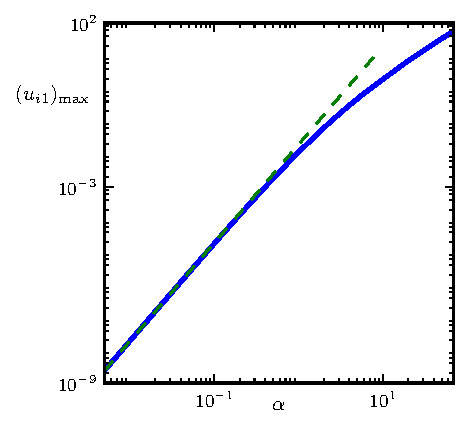
\includegraphics{Fig10}}
        \end{subfloatrow}\\[6pt]
        \begin{subfloatrow}
            \fcapside[\FBwidth]{\vspace{-10pt}\caption{}\label{fig:profile:qx}}{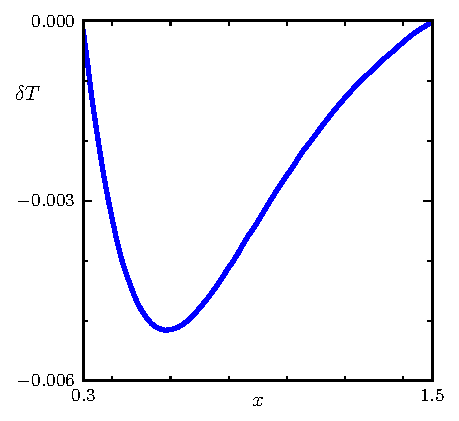
\includegraphics{Fig11}}
            \hspace{-20pt}
            \fcapside[\FBwidth]{\vspace{-10pt}\caption{}\label{fig:profile:qy}}{\includegraphics{Fig12}}
        \end{subfloatrow}\\[6pt]
        \begin{subfloatrow}
            \fcapside[\FBwidth]{\vspace{-10pt}\caption{}\label{fig:profile:P}}{\includegraphics{Fig13}}
            \hspace{-20pt}
            \fcapside[\FBwidth]{\vspace{-10pt}\caption{}\label{fig:profile:Pyy}}{\includegraphics{Fig14}}
        \end{subfloatrow}\\[6pt]
        \begin{subfloatrow}
            \fcapside[\FBwidth]{\vspace{-10pt}\caption{}\label{fig:profile:Pxx}}{\includegraphics{Fig15}}
            \hspace{-20pt}
            \fcapside[\FBwidth]{\vspace{-10pt}\caption{}\label{fig:profile:Pzz}}{\includegraphics{Fig16}}
        \end{subfloatrow}
    }{\phantomcaption}
\end{figure}
\begin{figure}
    \ContinuedFloat
    \ffigbox{
        \begin{subfloatrow}
            \fcapside[\FBwidth]{\vspace{-10pt}\caption{}\label{fig:profile:tau}}{\includegraphics{Fig17}}
            \hspace{-20pt}
            \fcapside[\FBwidth]{\vspace{-10pt}\caption{}\label{fig:profile:omega}}{\includegraphics{Fig18}}
        \end{subfloatrow}
    }{
        \vspace{-10pt}
        \caption{The profiles of the macroscopic variables.}
        \label{fig:profiles}
    }
\end{figure}

Fig.~\ref{fig:profiles} shows the profiles of the macroscopic variables.
Note some of their features.
Due to a growth in the gas pressure, the relative slip of the gas along the plate decreases
with increasing its speed (see also the asymptotic solution~\eqref{eq:Hilbert_U}).
The temperature jump decreases in the same way.
In the linear case, the longitudinal heat-flow vector \(q_x\) is presented only in the Knudsen layer,
but due to the strong anisotropy of the distribution function at large \(\Delta{v}\),
its bulk component increases faster than \((\Delta{v})^2\).
Therefore, the curvature of the profile \(q_x\) changes its sign with increasing \(\Delta{v}\).
The asymptotic solution describes the same behaviour for \(q_x\) (see Eq.~\eqref{eq:Hilbert_Qx}).
Owing to the significant heating of the gas at large \(\Delta{v}\),
the transverse heat-flow vector \(q_y\) grows faster than \((\Delta{v})^2\) too,
but the curvature of the profile preserves its sign.
Furthermore, depending on the \(\Delta{v}\) and \(\Kn\), \(q_x\) prevails over \(q_y\) at most.
The longitudinal stress \(P_{xx}\) is always greater than \(P_{yy}\) and \(P_{zz}\).
In the Knudsen layer, for small \(\Kn\), the constant stress \(P_{yy}\) becomes more than \(P_{zz}\).
Note that \(P_{ij}\) is not a shear stress tensor but a perturbed stress tensor
(see Eqs.~\eqref{eq:perturbed_variables}).
The temperature of the gas increases with \(\Kn\), because more rarefied gas
has a lower thermal conductivity.

\begin{figure}
    \centering
    \includegraphics{Fig19}
    \caption{The dependence of the shear stress on the Knudsen number.}
    \label{fig:shear}
\end{figure}

\begin{figure}
    \centering
    \includegraphics{Fig20}
    \caption{The dependence of the longitudinal mass flow on the Knudsen number.}
    \label{fig:flow}
\end{figure}

\begin{figure}
    \centering
    \includegraphics{Fig21}
    \caption{The dependence of the longitudinal heat flow on the Knudsen number.}
    \label{fig:qflow}
\end{figure}

\begin{figure}
    \centering
    \includegraphics{Fig22}
    \caption{The dependence of the transverse heat flow on the Knudsen number.}
    \label{fig:qflowy}
\end{figure}

\begin{figure}
    \centering
    \includegraphics{Fig23}
    \caption{The dependence of the difference \(P_{xx}-P_{yy}\) on the Knudsen number.}
    \label{fig:pxx}
\end{figure}

\begin{figure}
    \centering
    \includegraphics{Fig24}
    \caption{The dependence of the difference \(P_{zz}-P_{yy}\) on the Knudsen number.}
    \label{fig:pzz}
\end{figure}

\begin{figure}
    \centering
    \includegraphics{Fig25}
    \caption{The dependence of the temperature distribution on the Knudsen number.}
    \label{fig:temp}
\end{figure}

\begin{figure}
    \centering
    \includegraphics{Fig26}
    \caption{The absolute difference between solutions \(|\int_0^{1/2} (h^{(1)}-h^{(2)})\dd{y}|\),
        where \(h = P_{xy}, q_x, \tau\) and the superscript denotes the method, versus the Knudsen number:
        the lines without circles correspond to the asymptotic and projection-method solutions,
        the lines with circles correspond to the DSMC and projection-method solutions.}
    \label{fig:diff}
\end{figure}

Figs.~\ref{fig:shear}---\ref{fig:temp} show the macroscopic variables,
integrated over half of the volume between the plates \(0<y<1/2\), in dependence on the Knudsen number.
To depict the difference between results clearer,
we subtract the asymptotic solutions in two limits: \(\Kn\to0\) and \(\Kn\to\infty\),
and use the logarithmic scale.
The quantities with an asterisk are computed from the Navier--Stokes equations~\eqref{eq:Navier-Stokes}
with the nonslip boundary conditions~\eqref{eq:nonslip_bc}:
\begin{gather*}
    P_{\NS xy}^* = \frac1k \int_0^\frac12 P_{xy} \dd{y}, \quad P_{\NS xy} = P_{\NS xy}^*(\Delta{v}\to0) = -\gamma_1\frac{\Delta{v}}2, \\
    v_{\NS x}^* = \int_0^\frac12 v_x \dd{y}, \quad v_{\NS x} = v_{\NS x}^*(\Delta{v}\to0) = \frac{\Delta{v}}8, \\
    \tau_{\NS}^* = \int_0^\frac12 \tau \dd{y}, \quad
        \tau_{\NS} = \tau_{\NS}^*(\Delta{v}\to0) = \frac{\gamma_1}{\gamma_2}\frac{(\Delta{v})^2}{30}.
\end{gather*}
Their numerical values are shown in Tab.~\ref{table:NS_params}.

\begin{table}
    \centering
    \begin{tabular}{cccc}
        \(\Delta{v}\) & \(\displaystyle P_{\NS xy}^*/P_{\NS xy}\) & \(\displaystyle v_{\NS x}^*/v_{\NS x}\) & \(\displaystyle \tau_{\NS}^*/\tau_{\NS}\) \\[3pt]
        0.1 & 1.000220 & 0.999945 & 1.000049 \\
          1 & 1.021740 & 0.994715 & 1.004237 \\
          2 & 1.083898 & 0.981103 & 1.015173 \\
          5 & 1.438344 & 0.931106 & 1.055818 \\
    \end{tabular}
    \caption{Quantities obtained from the numerical solution of the Navier--Stokes equations.}
    \label{table:NS_params}
\end{table}

Figs.~\ref{fig:shear}---\ref{fig:qflow} show the macroscopic variables
that are not equal to zero in the linearized problem.
For small \(\Delta{v}\), verification of the results can be based
on the comparison with the accurate numerical solution of
the linearized Boltzmann equation~\citep{Ohwada1990} (the black line).
In contrast to the DSMC method, the numerical fluctuations in the projection-interpolation method
decrease when the flow approaches to the linear case (due to the power interpolation~\eqref{eq:ci_interpolation}).
Linear flows require less computational cost for the projection-interpolation method,
therefore, it is easy to compute a case of smaller \(\Delta{v}\) by the projection method,
but it is missed to save space in figures.

For comparison with the solution of the BKW equation (the cyan line),
\(k\) is replaced in~\eqref{eq:bkw_solution} by the following quantities:
\(\gamma_1k\) in Fig.~\ref{fig:shear},~\ref{fig:flow} and \(\gamma_2k\) in Fig.~\ref{fig:qflow}.
With this modification, the transport coefficients of viscosity and thermal conductivity
of the BKW solution coincide with the hard-sphere ones, because \(\gamma_1=\gamma_2=1\) for the BKW model.

In Fig.~\ref{fig:shear} and Fig.~\ref{fig:qflow}, the difference between the asymptotic (the blue line)
and projection-method (the red line) solutions is \(\OO{\Kn^3}\),
which is in accordance with Eq.~\eqref{eq:Hilbert_Pxy} and Eq.~\eqref{eq:Hilbert_Qx}.
For \(\Delta{v}=0.1\), the asymptotic solution is close to the linear one~\eqref{eq:linear_macro},
which has the larger order of the approximation.
In Fig.~\ref{fig:flow}, the deviation of the projection-method curves
from the asymptotic solution for small \(\Kn\) indicates that
the error of the projection-method solution is within the interval from \(10^{-5}\) to \(10^{-4}\).
These facts are more evident in Fig.~\ref{fig:diff},
where the absolute difference between the solutions
is depicted for some macroscopic variables.
The increase of the error for \(\tau\) and \(v_x\) for the smallest \(\Kn\)
is due to the insufficient number of time steps performed during the simulation.
In other words, the steady state is not reached completely.

The DSMC method (the green line) produces an error within the interval from \(10^{-4}\) to \(10^{-3}\),
mainly due to large fluctuations, especially for \(\Delta{v}=0.1\).
In Fig.~\ref{fig:shear}, there is a constant-sign difference
between the DSMC and projection-method solutions.
It can be reduced with the time step tending to zero.
A smaller time step is intentionally not employed in the present DSMC computation
to illustrate that even so small time step as~\eqref{eq:dsmc_timestep} can be insufficient
to achieve a high-accuracy solution.
Incidentally, other quantities, calculated by DSMC, are not shifted with
a further reduction in the time step.

Figs.~\ref{fig:qflowy}---\ref{fig:temp} show the macroscopic variables
arising as a square of the \(\Delta{v}\).
Results for \(\Delta{v}=0.1\) are omitted due to low precision.
The difference between the asymptotic and projection-method solutions
is \(\OO{\Kn^3}\) in Fig.~\ref{fig:qflowy}--\ref{fig:pzz} and \(\OO{\Kn^2}\) in Fig.~\ref{fig:temp}.
Taking into account the accuracy of individual approaches,
all presented results are in good agreement.

\section{Concluding remarks}

%%% A little bit about results
By means of the direct numerical solution of the Boltzmann equation using the projection-interpolation method,
an error of about \(10^{-4}\) has been achieved for a wide range of the external parameters:
\(0.01 \le \Kn \le 100\) and \(0.1 \le \Delta{v} \le 5\).
The presented set of the profiles for the first thirteen moments demonstrates
the main features of the plane Couette flow in dependence of \(\Kn\) and \(\Delta{v}\).
The latter dependence is of particular interest due to poor coverage in the literature.
For instance, the curvature of the profile of the longitudinal heat-flow vector
changes its sign with increasing \(\Delta{v}\).
This fact is usually not mentioned in other papers.
In the present study, the complete diffuse reflection is used as the kinetic boundary condition
for the sake of simplicity. The real experiments show that the accommodation coefficient
is close to unity but slightly differs from it~\citep{Agrawal2008}.

%%% Asymptotic analysis, its connection to NS equations
In the context of the plane Couette-flow problem,
a comparative analysis of the applied numerical methods can be carried out.
For small \(\Kn\), the asymptotic analysis of the Boltzmann equation has demonstrated
its superiority in terms of accuracy and performance.
The derived fluid-dynamic-type equations, coinciding with the Navier--Stokes equations,
together with the appropriate nonlinear slip boundary conditions (presented by~\citet{Sone2000})
and the Knudsen-layer correction, allow to obtain a solution with error \(\OO{\Kn^2}\).
Note that the expressions for the deviatoric stress tensor and heat-flow vector
differ from the Newton's and Fourier's laws and have an error \(\OO{\Kn^3}\).
They contain the additional transport coefficients besides the viscosity and thermal conductivity ones,
which have been computed in the present paper for the hard-sphere model.
However, in the general asymptotic theory, the situation is not so promising.
First, the expansion parameter in the viscous boundary layer is \(\sqrt{\Kn}\) (in contrast to \(\Kn\)).
Second, the asymptotic analysis in curvilinear coordinates leads to the cumbersome expressions~\citep{Sone2002}.
Finally, if the viscous boundary layer is not smooth,
the method of constructing the asymptotic solution is not obvious~\citep{Aoki2014}.

%%% Comparison of accuracy between the projection method and DSMC
For discrete-velocity methods, there is a typical problem to obtain a high-accuracy solution:
the appropriate discretization of velocity space should be constructed
to provide a satisfactory approximation of the distribution function.
Stochastic techniques do not have such complications,
but at the same time have slow convergence rate of \(\OO{N^{-1/2}}\)
(\(N\) is a total number of particles)
for both smooth and discontinuous distribution functions.
In contrast, the projection method, under an appropriate discretization,
has a satisfactory convergence of \(\OO{N^{-1}}\)
(\(N\) is a total number of integration lattice points)
for a discontinuous distribution function and \(\OO{N^{-2}}\) for the smooth one.
For the rather simple plane Couette-flow problem,
the DSMC method yields a quite good accuracy, but its statistical noise
is an order of magnitude greater than within the discrete-velocity solution, even for finite \(\Delta{v}\).
Incidentally, the low-variance DSMC method~\citep{Hadji2011}
can be applied to decrease an enormous statistical error for small \(\Delta{v}\),
where fluctuations are especially large in comparison with the solution.

%%% Comparison of performance between the projection method and DSMC
Finally, it is necessary to mention performance of the methods.
In the present study, a direct numerical solution of the Boltzmann equation, on average,
took an order of magnitude more time than the statistical simulation.
However, for coarser grids and integration lattice, the projection method can
have better performance with the same accuracy as that of the DSMC method.
Moreover, for complex \textit{ab initio} molecular potentials, computational costs are almost not increased~\citep{Dodulad2014},
while simplified model potentials (e.g. variable hard spheres) have to be used in the DSMC method.
In fact, discrete-velocity methods have high performance on fixed velocity grids,
which are identical in each physical cell.
In a general case, the fixed velocity grid should be uniform or close to it and, therefore,
should be sufficiently fine to approximate large variations of the distribution function accurately.
This requirement can be very costly. An alternative approach is to use adaptive velocity grids~\citep{Kolobov2013}.

%%% Perspectives
In view of the above discussion, the proposed projection method on nonuniform grids can be recommended
for solving nonlinear boundary-value problems with high accuracy.

\section*{Acknowledgement}

The author is grateful to Dr. Oleg Dodulad, who implements the extension
of the projection method for the nonuniform velocity grids,
and Dr. Felix Tcheremissine for his valuable comments.

\appendix
\section{The transport coefficients \(\gamma_8\), \(\gamma_9\) and \(\gamma_{10}\)}
\label{sec:gamma_coeffs}

The general formulas for calculation \(\gamma_8\), \(\gamma_9\) and \(\gamma_{10}\)
for hard-sphere molecules are~\citep{Sone2000, Sone2002, Sone2007}
\begin{gather}
    \gamma_8 = I_6\left(\Q_2 - \QQ_{22}\right) + \frac17 I_8\left(\Q_3 - \QQ_3\right), \label{eq:gamma_8}\\
    \gamma_9 = -I_6\left(\B\right), \label{eq:gamma_9}\\
    \gamma_{10} = \frac58 I_6\left(\T{1}_1 + \T{2}_1 - 2\TT_{12}\right)
        + \frac18 I_8\left(\T{1}_2 + \T{2}_2 - 2\TT_2\right), \label{eq:gamma_10}
\end{gather}
where,
\begin{equation}\label{eq:I_n}
    I_n[Z(\zeta)] = \frac{8}{15\sqrt{\pi}} \int_0^\infty \zeta^n Z(\zeta) \exp(-\zeta^2) \dd\zeta.
\end{equation}
The integrands can be obtained from the corresponding integral equations:
\begin{align}
    \mathcal{L}\left(\zeta_x\mathcal{A}\right) &= -\zeta_x\left(\zeta^2-\frac52\right), \label{eq:A}\\
    \mathcal{L}\left(\zeta_x\zeta_y\mathcal{B}\right) &= -2\zeta_x\zeta_y, \label{eq:B}\\
    \mathcal{L}\left(\zeta_x\zeta_y\B\right) &= \zeta_x\zeta_y\mathcal{B}, \label{eq:B_4}
\end{align}
\begin{align}
    \mathcal{L}\left( \zeta_x\zeta_y\zeta_z\T{1}_2 \right)
        &= -\zeta_x\zeta_y\zeta_z\left(2\mathcal{A} - \frac1\zeta\der[\mathcal{A}]{\zeta}\right), \label{eq:T2a}\\
    \mathcal{L}\left[ \zeta_x\left(3\T{1}_1 + \zeta_x^2\T{1}_2\right) \right]
        &= -\zeta_x^3\left(2\mathcal{A} - \frac1\zeta\der[\mathcal{A}]{\zeta}\right), \label{eq:T1a}\\
    \mathcal{L}\left( \zeta_x\zeta_y\zeta_z\T{2}_2 \right)
        &= -\zeta_x\zeta_y\zeta_z\left((\zeta^2-3)\mathcal{B} - \frac\zeta2\der[\mathcal{B}]{\zeta}\right), \label{eq:T2b}\\
    \mathcal{L}\left[ \zeta_x\left(3\T{2}_1 + \zeta_x^2\T{2}_2\right) \right]
        &= -\zeta_x^3\left((\zeta^2-3)\mathcal{B} - \frac\zeta2\der[\mathcal{B}]{\zeta}\right) + \frac{3\gamma_1}{2}\zeta_x, \label{eq:T1b}\\
    \mathcal{L}\left( \zeta_x\zeta_y\zeta_z\TT_2 \right)
        &= \mathcal{J}\left( \zeta_x\mathcal{A}, \zeta_y\zeta_z\mathcal{B} \right), \label{eq:TT2}\\
    \mathcal{L}\left[ \zeta_y\left(\TT_{12} + \zeta_x^2\TT_2\right) \right]
        &= \mathcal{J}\left( \zeta_x\mathcal{A}, \zeta_x\zeta_y\mathcal{B} \right), \label{eq:TT12}
\end{align}
\begin{align}
    \mathcal{L}\left[ \zeta_x\zeta_y \left( 3\zeta_z^2-\zeta_x^2 \right)\Q_3 \right]
        &= -\zeta_x\zeta_y\left( 3\zeta_z^2-\zeta_x^2 \right)\left(2\mathcal{B} - \frac1\zeta\der[\mathcal{B}]{\zeta}\right), \label{eq:Q3}\\
    \mathcal{L}\left[ \zeta_x\zeta_y \left( 3\Q_2+\zeta_x^2\Q_3 \right) \right]
        &= -\zeta_x^3\zeta_y\left(2\mathcal{B} - \frac1\zeta\der[\mathcal{B}]{\zeta}\right), \label{eq:Q2}\\
    \mathcal{L}\left[ \zeta_x\zeta_y\left( 3\zeta_z^2 - \zeta_x^2 \right)\QQ_3 \right]
        &= \mathcal{J}\left( \zeta_x\zeta_y\mathcal{B}, \zeta_z^2\mathcal{B} \right)
        + 2\mathcal{J}\left( \zeta_x\zeta_y\mathcal{B}, \zeta_x\zeta_z\mathcal{B} \right)
        - \mathcal{J}\left( \zeta_x\zeta_y\mathcal{B}, \zeta_x^2\mathcal{B} \right), \label{eq:QQ3}\\
    \mathcal{L}\left[ \zeta_x\zeta_y \left( \QQ_{22} + \zeta_z^2\QQ_3 \right) \right]
        &= \mathcal{J}\left( \zeta_x\zeta_y\mathcal{B}, \zeta_x\zeta_z\mathcal{B} \right) \label{eq:QQ2}
\end{align}
with subsidiary conditions for \(\mathcal{A}\), \(\T{m}_1\), \(\TT_{12}\):
\begin{gather}
    \int_0^\infty \zeta^4 \mathcal{A} E \dd\zeta = 0, \label{eq:A_constraint}\\
    \int_0^\infty \left( 5\zeta^4\T{m}_1 + \zeta^6\T{m}_2 \right) E \dd\zeta = 0, \label{eq:Tm_constraint}\\
    \int_0^\infty \left( 5\zeta^4\TT_{12} + \zeta^6\TT_2 \right) E \dd\zeta = 0. \label{eq:T12_constraint}
\end{gather}
The collision operators \(\mathcal{L}\) and \(\mathcal{J}\) are related to the collision integral \(J\) as follows:
\begin{equation}\label{eq:mathcalLJ}
    E\mathcal{L}(\phi) = 2J(1, E\phi), \quad E\mathcal{J}(\phi, \psi) = J(E\phi, E\psi).
\end{equation}

The integral equations~\eqref{eq:A}--\eqref{eq:B} can be solved accurately
by reducing them to ordinary differential equations~\citep[see e.g.][]{Pekeris1957, Ohwada1992}.
For the present paper, the considered integral equations are solved
by the fixed-point iteration and direct quasi-Monte Carlo integration.
The desired functions are shown in Fig.~\ref{fig:transport_functions}.

\begin{figure}
    \centering
    \begin{subfigure}[b]{0.33\textwidth}
        \includegraphics[right]{Fig27}
        \label{fig:B}
    \end{subfigure}%
    \begin{subfigure}[b]{0.33\textwidth}
        \includegraphics[right]{Fig28}
        \label{fig:B_4}
    \end{subfigure}%
    \begin{subfigure}[b]{0.33\textwidth}
        \includegraphics[right]{Fig29}
        \label{fig:T1_1}
    \end{subfigure}\\[-6pt]
    \begin{subfigure}[b]{0.33\textwidth}
        \includegraphics[right]{Fig30}
        \label{fig:T1_2}
    \end{subfigure}%
    \begin{subfigure}[b]{0.33\textwidth}
        \includegraphics[right]{Fig31}
        \label{fig:T2_1}
    \end{subfigure}%
    \begin{subfigure}[b]{0.33\textwidth}
        \includegraphics[right]{Fig32}
        \label{fig:T2_2}
    \end{subfigure}\\[-6pt]
    \begin{subfigure}[b]{0.33\textwidth}
        \includegraphics[right]{Fig33}
        \label{fig:TT12}
    \end{subfigure}%
    \begin{subfigure}[b]{0.33\textwidth}
        \includegraphics[right]{Fig34}
        \label{fig:TT2}
    \end{subfigure}%
    \begin{subfigure}[b]{0.33\textwidth}
        \includegraphics[right]{Fig35}
        \label{fig:Q2}
    \end{subfigure}\\[-6pt]
    \begin{subfigure}[b]{0.33\textwidth}
        \includegraphics[right]{Fig36}
        \label{fig:Q3}
    \end{subfigure}%
    \begin{subfigure}[b]{0.33\textwidth}
        \includegraphics[right]{Fig37}
        \label{fig:QQ22}
    \end{subfigure}%
    \begin{subfigure}[b]{0.33\textwidth}
        \includegraphics[right]{Fig38}
        \label{fig:QQ3}
    \end{subfigure}\\[-6pt]
    \caption{The transport functions for hard-sphere molecules.}
    \label{fig:transport_functions}
\end{figure}

\bibliography{manuscript}
\bibliographystyle{elsarticle-num-names}

\end{document}

